\documentclass[12pt,a4paper]{article}
\usepackage{geometry}
\newgeometry{tmargin=2cm, bmargin=2cm, lmargin=2cm, rmargin=2cm}
\usepackage[polish]{babel}
\usepackage[T1]{fontenc}
\usepackage[utf8]{inputenc}
\usepackage{amsmath}
\usepackage[dvips]{graphicx}
\usepackage{listings}                       % pakiet wymagany do otoczenia lstlisting
\usepackage[usenames,dvipsnames]{xcolor}    % wymagane do definicji własnych kolorów
\definecolor{mygreen}{RGB}{25,130,0}        % definicja koloru
\definecolor{mylilas}{RGB}{180,55,230}      % definicja koloru
\definecolor{myNumbers}{RGB}{180,222,230}   
\usepackage{amsmath}
\begin{document}
\lstloadlanguages{Matlab}                   
\lstset{language=Matlab,                    
    breaklines=true,
    basicstyle=\ttfamily,%
    columns=fullflexible,%
    extendedchars=true,%
    inputencoding=utf8,%
    showstringspaces=false%
    keepspaces=true,
    morekeywords={matlab2tikz},
    keywordstyle=\color{blue},
    morekeywords=[2]{1},
    keywordstyle=[2]{\color{black}},
    identifierstyle=\color{black},
    stringstyle=\color{mylilas},
    commentstyle=\color{mygreen},
    showstringspaces=false,
    emph=[1]{if,while,for,end,break},
    emphstyle=[1]\color{red},
	tabsize=2,
    xleftmargin=2em,
    frame=single,
    framexleftmargin=1.5em,
}

\section*{Zadanie 3}

Narysować wykres funcji

\[
z = f(x, y) = \frac{1}{2\pi \sigma_x \sigma_y} 
\exp\left( 
-\frac{(x - x_0)^2}{2\sigma_x^2} 
- \frac{(y - y_0)^2}{2\sigma_y^2} 
\right)
\]

\vspace{1em}

dla $\sigma_x$, $\sigma_y$ wygenerowanych losowo w przedziale $[1, 2]$ oraz $x_0 = y_0 = 0$.

\vspace{1em}

\begin{lstlisting}

%praca domowa 3

x_0 = 0;
y_0 = 0;
a = 1;
b = 2;

sigma_x = 1 + (b-a)*rand;
sigma_y = 1 + (b-a)*rand;

x = linspace(-3*max(sigma_x,1), 3*max(sigma_x,1), 100);
y = linspace(-3*max(sigma_y,1), 3*max(sigma_y,1), 100);

[X, Y] = meshgrid(x,y);

Z = 1/(2*pi*sigma_x*sigma_y) * exp(...
    -((X-x_0).^2)/(2*sigma_x^2)-((Y - y_0).^2)/(2*sigma_y^2));

S = surf(X,Y,Z);
S.EdgeColor = 'none';
colormap hot;
colorbar;

xlabel('x');
ylabel('y');
zlabel('z = f(x,y)');

title({['\sigma_x = ', num2str(sigma_x, '%.3f'), ...
            ', \sigma_y = ', num2str(sigma_y, '%.3f'), ...
            ', x_0 = y_0 = 0']
           });

print -depsc wykres3.eps

\end{lstlisting}


\begin{figure}[h]
    \centering
    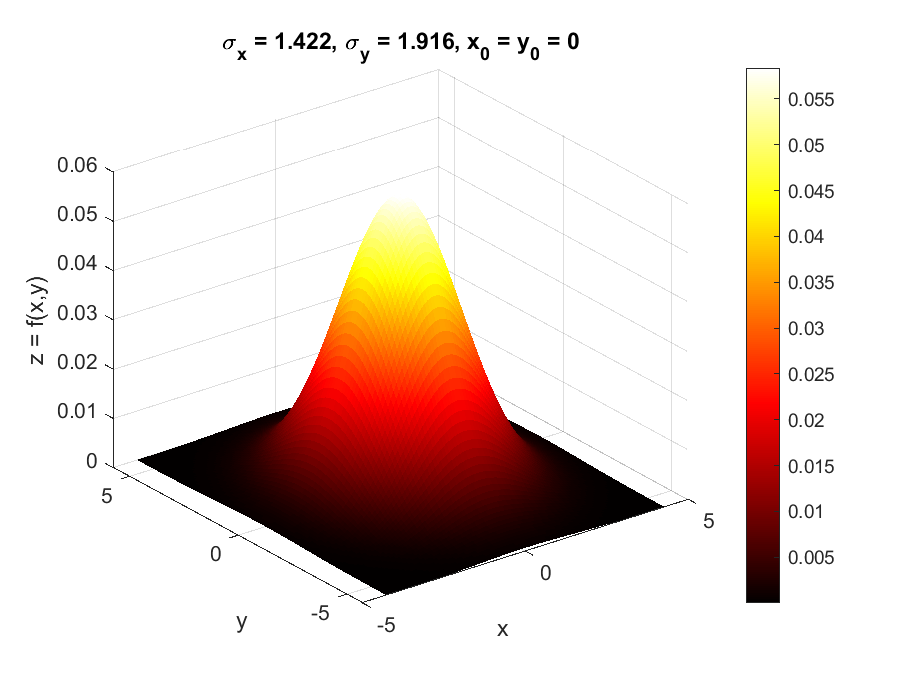
\includegraphics[width=0.8\textwidth]{wykres3.eps}
    \caption{Wykres funkcji:
    \begin{equation}
     z = f(x, y) = 
    \frac{1}{2\pi \sigma_x \sigma_y}
    \exp\left(
    -\frac{(x - x_0)^2}{2\sigma_x^2}
    - \frac{(y - y_0)^2}{2\sigma_y^2}
    \right)   
    \end{equation}}
    \label{fig:wykresy}
\end{figure}

\end{document}